

\title{Seismic Event MatLAB Suite (SEMS) Cookbook}                                                  
\author{Dane Ketner \\Alaska Volcano Observatory\\dketner@usgs.gov}
\date{\today}

\documentclass[11pt]{article}

\evensidemargin=2.0in
\oddsidemargin=-0.25in
\textwidth=7.0in
\topmargin=.2in
\headsep=0in
\headheight=-.25in
\headsep=0in
\textheight=9.7in

\usepackage{graphicx} 
\usepackage{setspace}
\usepackage{amsmath}
\usepackage{esint}
\usepackage{mcode}

\renewcommand{\topfraction}{0.85}
\renewcommand{\textfraction}{0.1}
\renewcommand{\floatpagefraction}{0.85}

\newenvironment{my_enumerate}{
\begin{enumerate}
  \setlength{\itemsep}{1pt}
  \setlength{\parskip}{0pt}
  \setlength{\parsep}{0pt}}{\end{enumerate}
}


\begin{document}

\maketitle

\clearpage

\tableofcontents

\clearpage

\section{Introduction to SEMS}

The Seismic Event MatLAB Suite is a collection of MatLAB classes, functions, and GUIs used to capture, manipulate, and display large numbers of discrete seismic events. SEMS is build upon the Waveform Suite and other classes found in the GISMO Suite. SEMS commonly references event times in following formats depending on the application:

\begin{enumerate}

\item[1] SST - Event Start/Stop Times, event times are listed as a Nx2 array of MatLAB datenum values. This is the bare bones format for tracking periods of interest from a given waveform. The SCNL object is the other piece needed to recover waveform data from SST format.

\item[2] WFA - Event Waveform Array, events are contained in a 1xN array of waveform objects. This is the neccessary format for most operations.

\item[3] NAN - Event NaN Form: Events are contained in a longer waveform object with non-event times filled with NaN values. This is a useful format primarily for plotting purposes.

\end{enumerate}

There are a handful of functions that quickly fascilitate conversion between these formats: 
\begin{itemize}
\item \mcode{sst2wfa}
\item \mcode{sst2nan}
\item \mcode{wfa2sst}
\item \mcode{wfa2nan}
\item \mcode{nan2sst}
\item \mcode{nan2wfa}
\end{itemize}
SEMS includes a few functions additionally that operate only on SST arrays including: 
\begin{itemize}
\item \mcode{add_sst}
\item \mcode{delete_sst}
\item \mcode{extract_sst}
\item \mcode{merge_sst}
\item \mcode{search_sst}
\item \mcode{sort_sst}
\item \mcode{compare_sst}
\end{itemize}

Typing \mcode{help function_name} for any of the functions discussed in this manual should reveal more specific information about its functionality. The functions in SEMS are designed to be both modular and customizeable.
\clearpage


\section{Helicorder Class}

A helicorder (or seismogram) is a multi-line display of ground motion traditionally recorded onto paper around a rotating drum. The MatLAB helicorder class is designed to generate such a multi-line display and includes a number of customizeable properties that can be defined by the user, or ignored. One can think of a helicorder object \mcode{h} as a blueprint for the construction of a helicorder figure. The \mcode{build} function is then used to create the helicorder figure based on the properties in \mcode{h}. User-defined properties can override default properties if included in a call to the heliorder constructor, though all that is needed for a basic helicorder is a single waveform object input argument. In the following example, \mcode{w} is a waveform object containing three hours of data from REF:EHZ starting from March 29, 2009 starting at 07:00 UTC. Figure~\ref{hel_single_1} displays the output of the \mcode{build} function, with \mcode{fh} being the handle of the figure generated.   

\begin{lstlisting}
h = helicorder(w);
fh = build(h);
\end{lstlisting}

We see that the resulting helicorder figure contains 10 minutes of data per line, and that waveform data is printed in black. Also notice the amplitude scaling that occurs in the plot. This scaling sets the max datapoint value at the center of the trace two traces above (or below) the current trace. The max value in this plot appears to be the first earthquake on line 6 (Line 07:50:00) which reaches up to the center of line 4 (Line 07:30:00). Minutes per line, trace color, and scale are all properties that can be manually set. A user-defined property can be set upon initial creation of \mcode{h} in the following way: \mcode{h = helicorder(w, 'mpl', 15);}. This call to the constructor would override the default value of 10 with 15 minutes per line. Property values can also be set after \mcode{h} is constructed using the \mcode{set} function as follows: \mcode{h = set(h, 'mpl', 15);}.

\begin{figure}[ht] 
\centerline{\scalebox{.4} {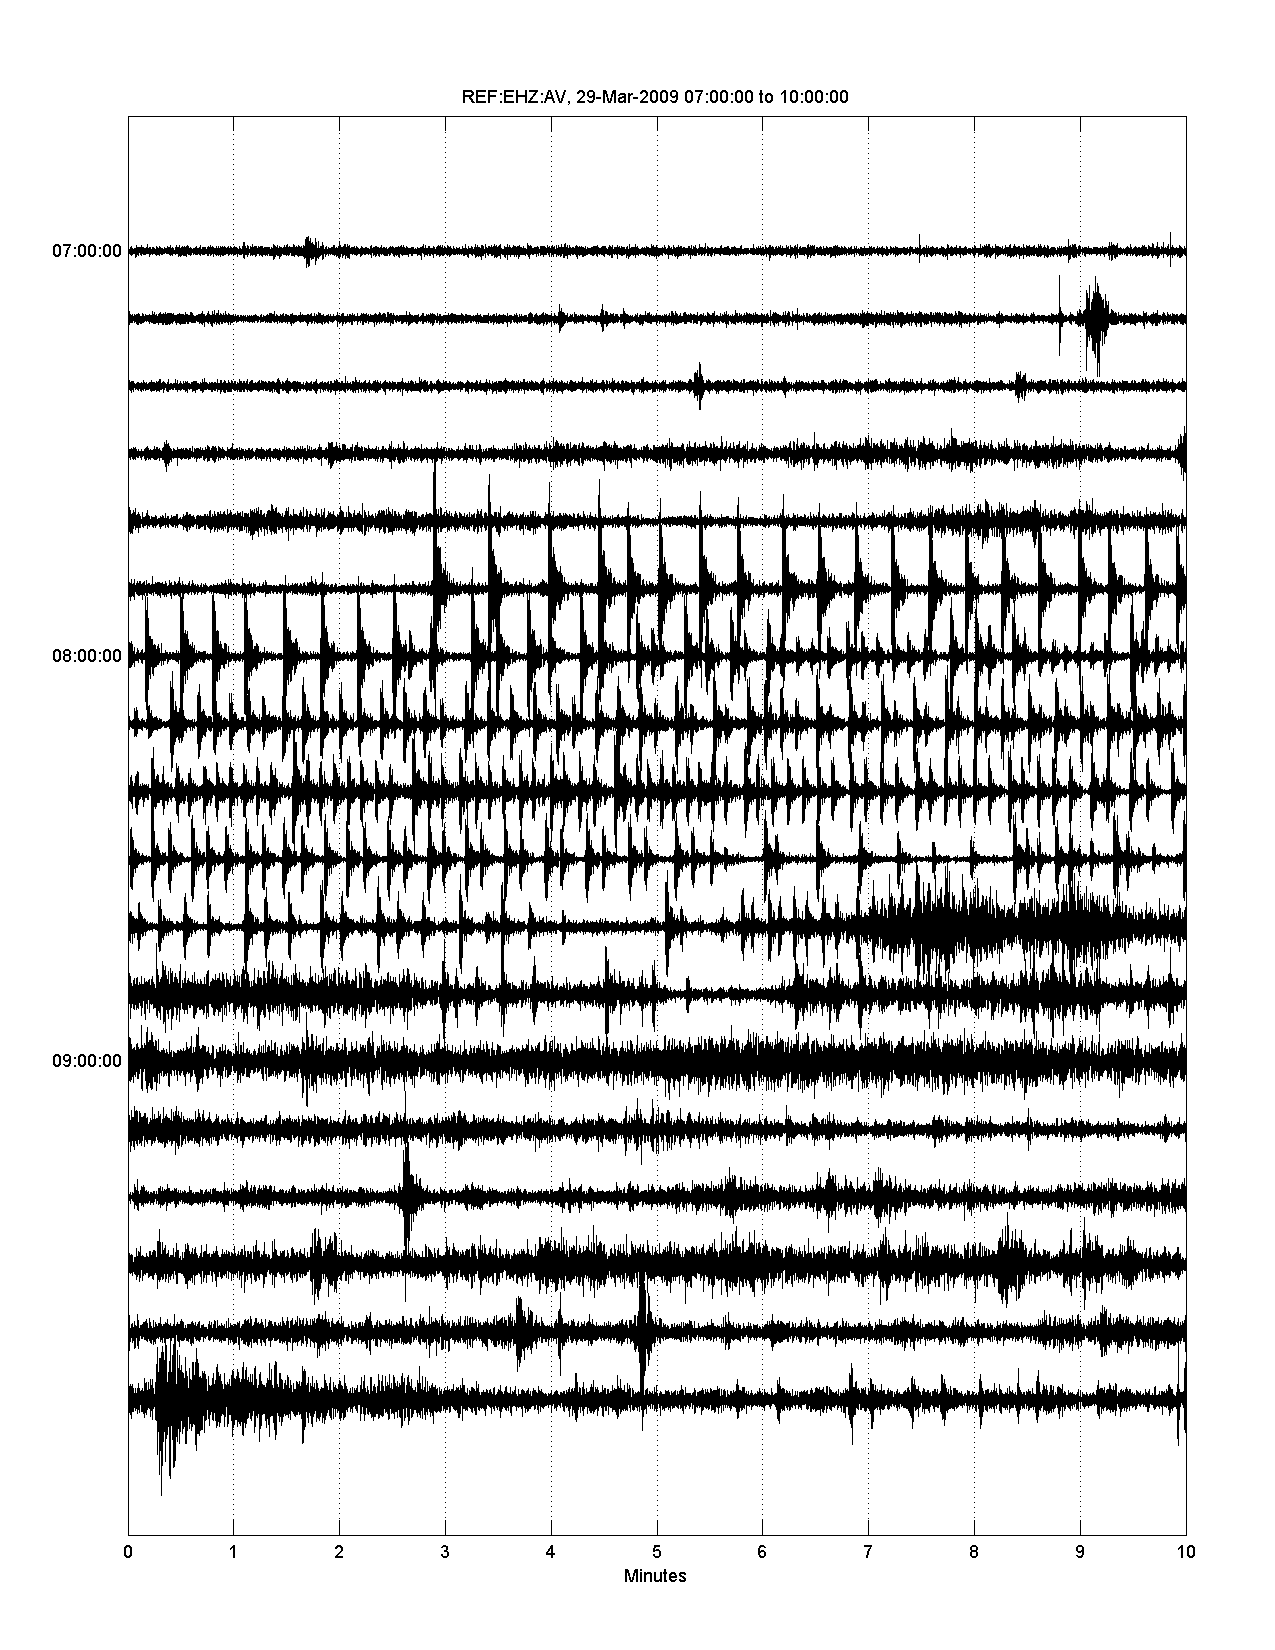
\includegraphics{hel_single_1.png}}} 
\caption{Default helicorder display for a single waveform} 
\label{hel_single_1}
\end{figure}
\clearpage

\subsection{Helicorder Multi-waveform display}

Next, let's test the default display created from an input \mcode{w} which contains multiple waveforms. In this case \mcode{w} is a 1x3 waveform object containing all three components from station REF for the same time span as the previous case. We know there will be more data to display than the previous example, so we set 20 minutes per line: \mcode{build(helicorder(w,'mpl',20))}. EHZ data is displayed in blue, EHE in black, and EHN in green in Figure~\ref{hel_alternate_1}. This multi-waveform display type is called 'alternate' which can be changed by the user in addition to the color scheme.

\begin{figure}[ht] 
\centerline{\scalebox{.6} {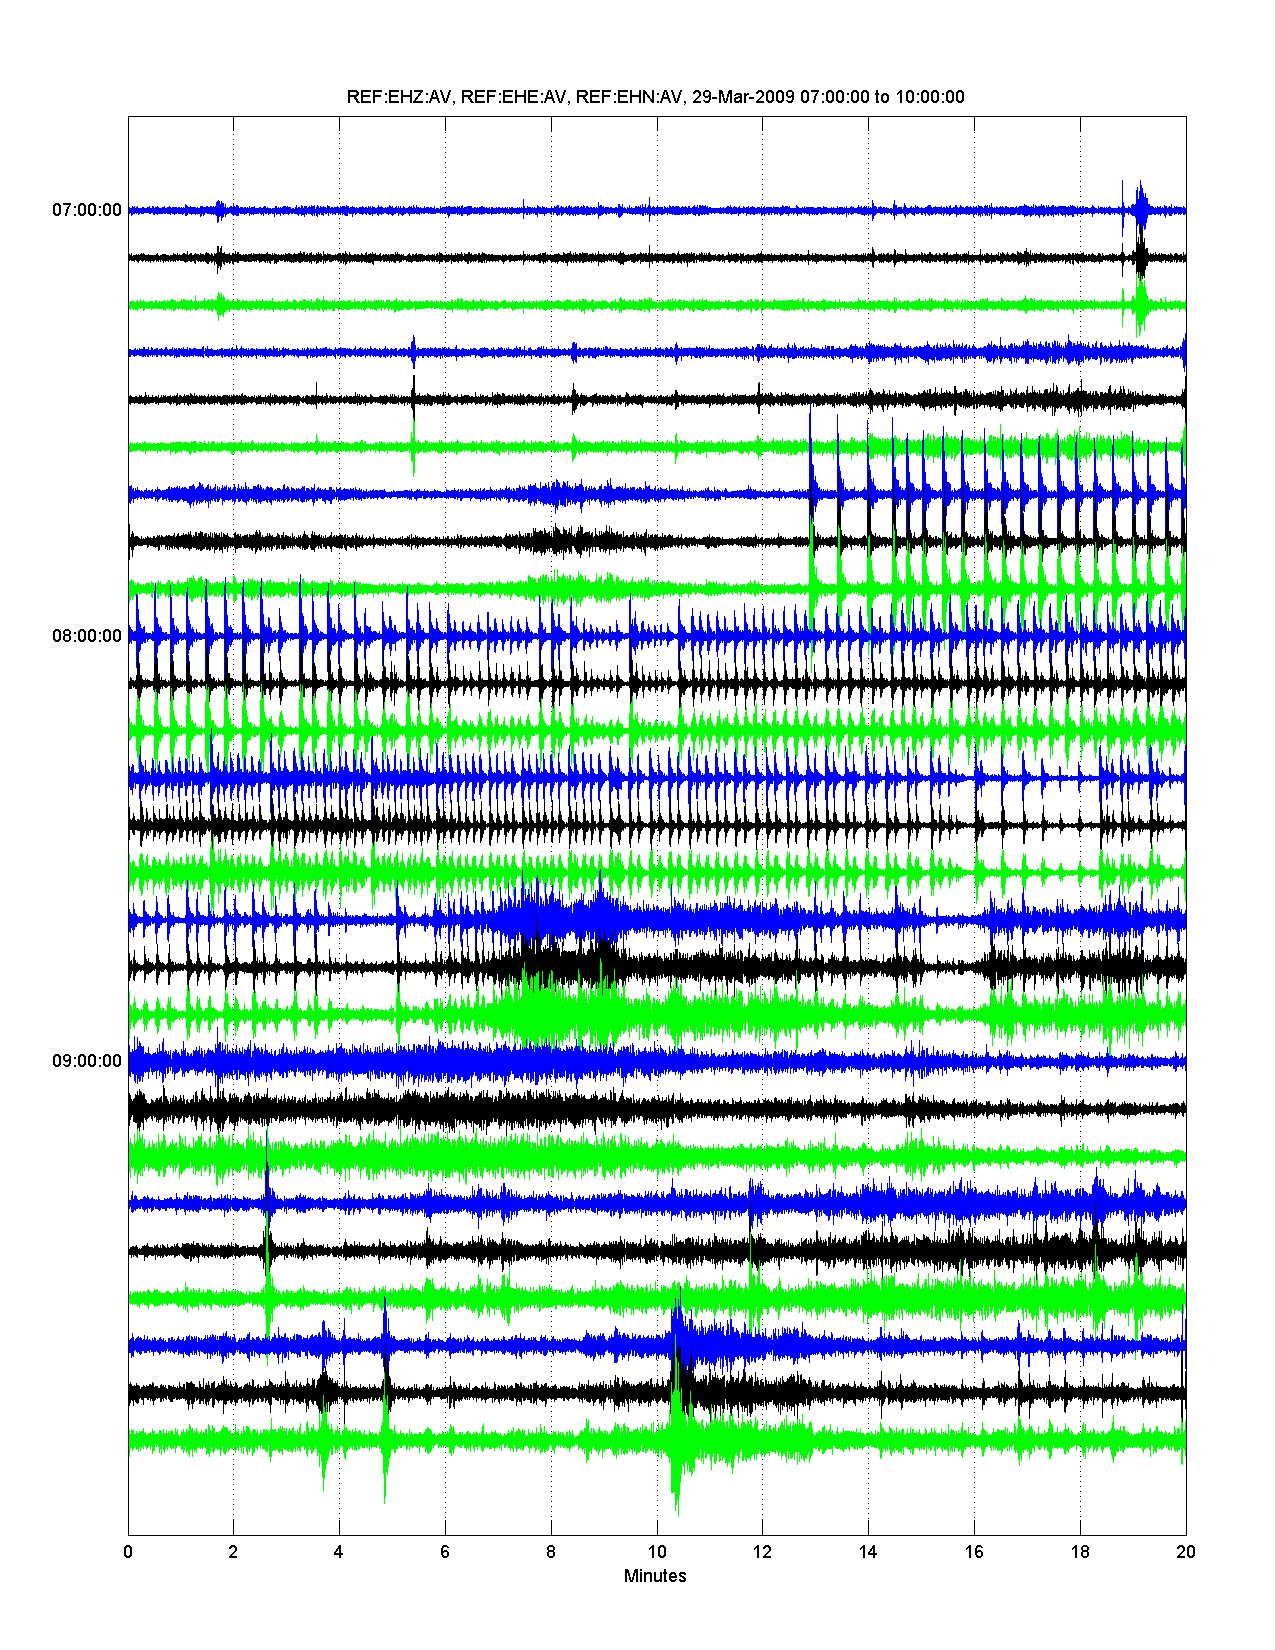
\includegraphics{hel_alternate_1.png}}} 
\caption{Default helicorder display for a 1x3 waveform} 
\label{hel_alternate_1}
\end{figure}
\clearpage

The multi-waveform display type can be changed from 'alternate' to 'group' or 'stack'. Setting display to 'group' will plot all trace data from the first element in \mcode{w} before starting the next. Figure~\ref{hel_group_1} displays the output from \mcode{build(helicorder(w,'mpl',20,'display','group'))}.

\begin{figure}[ht] 
\centerline{\scalebox{.6} {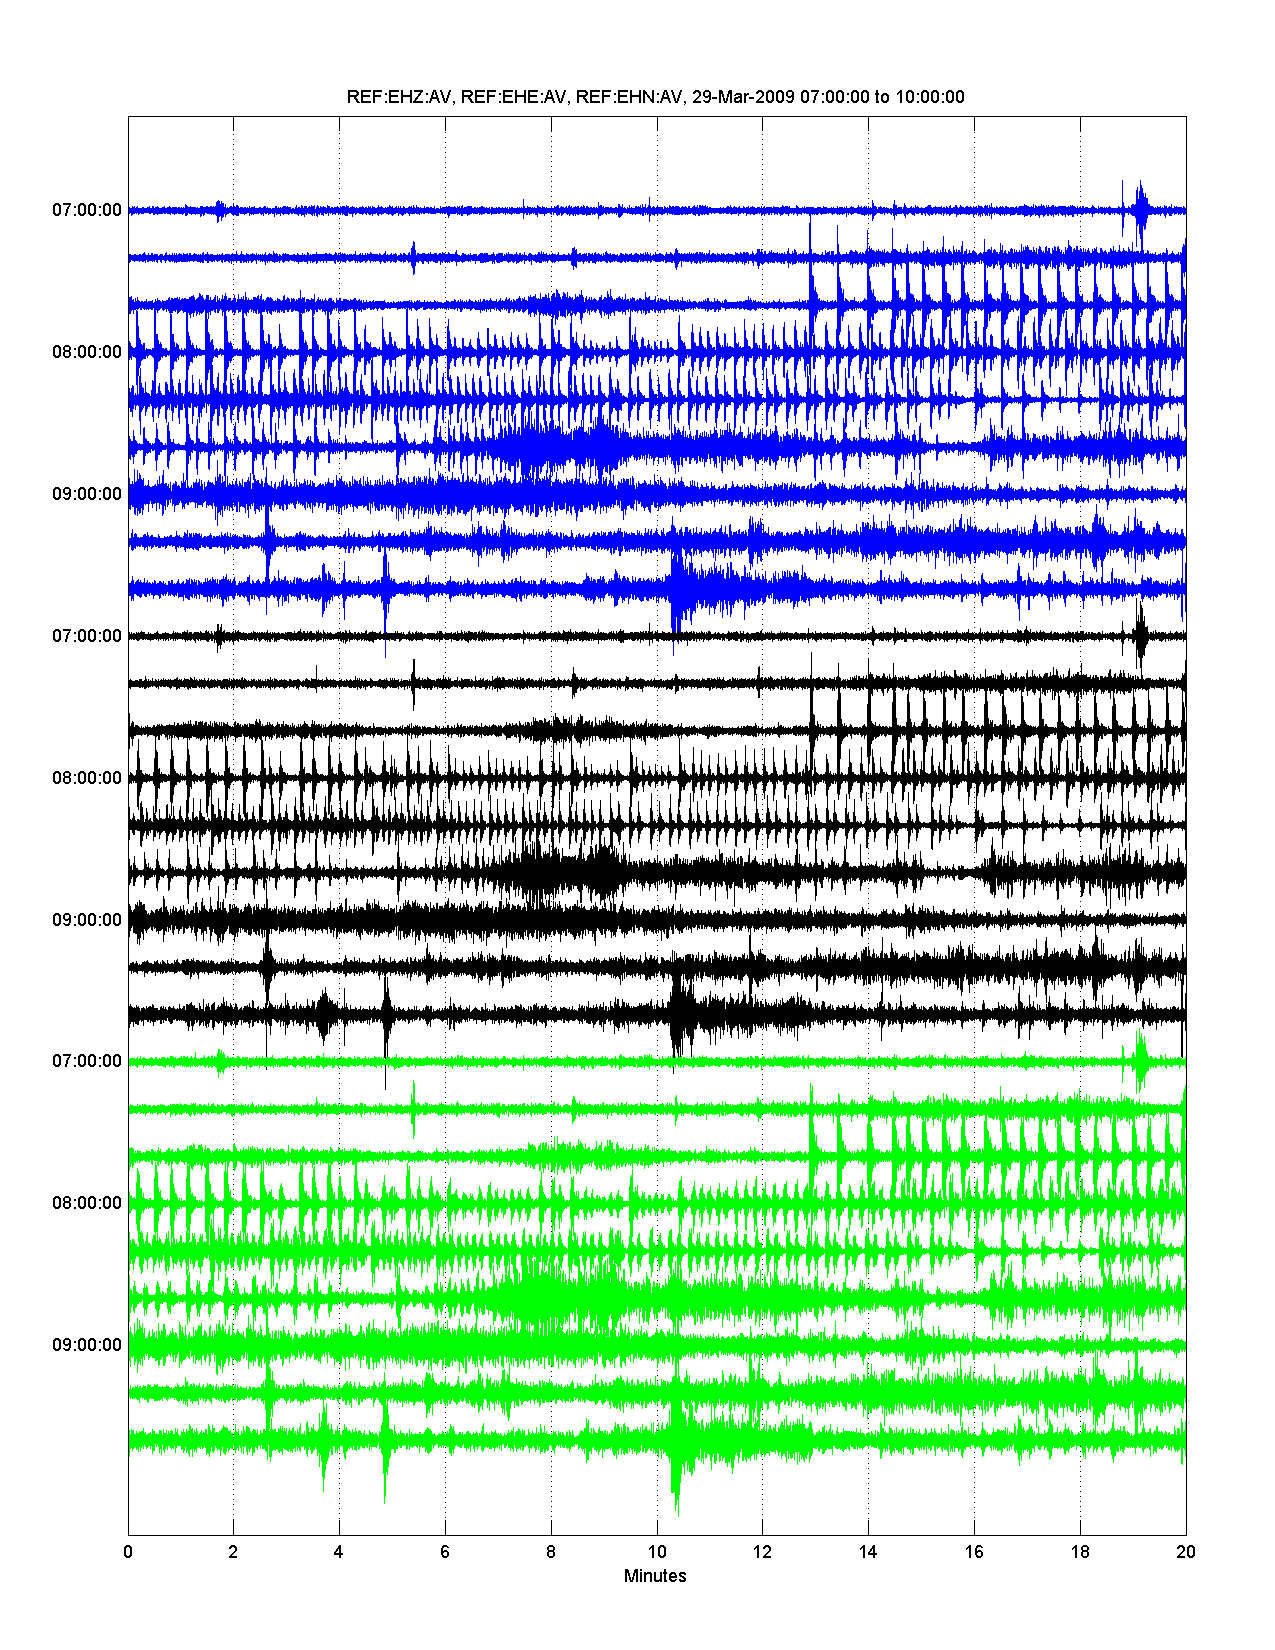
\includegraphics{hel_group_1.png}}} 
\caption{Multi-waveform 'group' display} 
\label{hel_group_1}
\end{figure}
\clearpage

The final multi-waveform display type is 'stack' which will plot waveforms one on top of the other. It should be noted that the default amplitude scaling of all waveforms is determined by the first waveform plotted in 'stack' mode, in this case \mcode{w(1)} is REF:EHZ. If separate amplitude scaling is desired for waveforms in w, it must be defined by the user. Figure~\ref{hel_stack_1} displays the output from \\ \mcode{build(helicorder(w,'display','stack'))}.

\begin{figure}[ht] 
\centerline{\scalebox{.6} {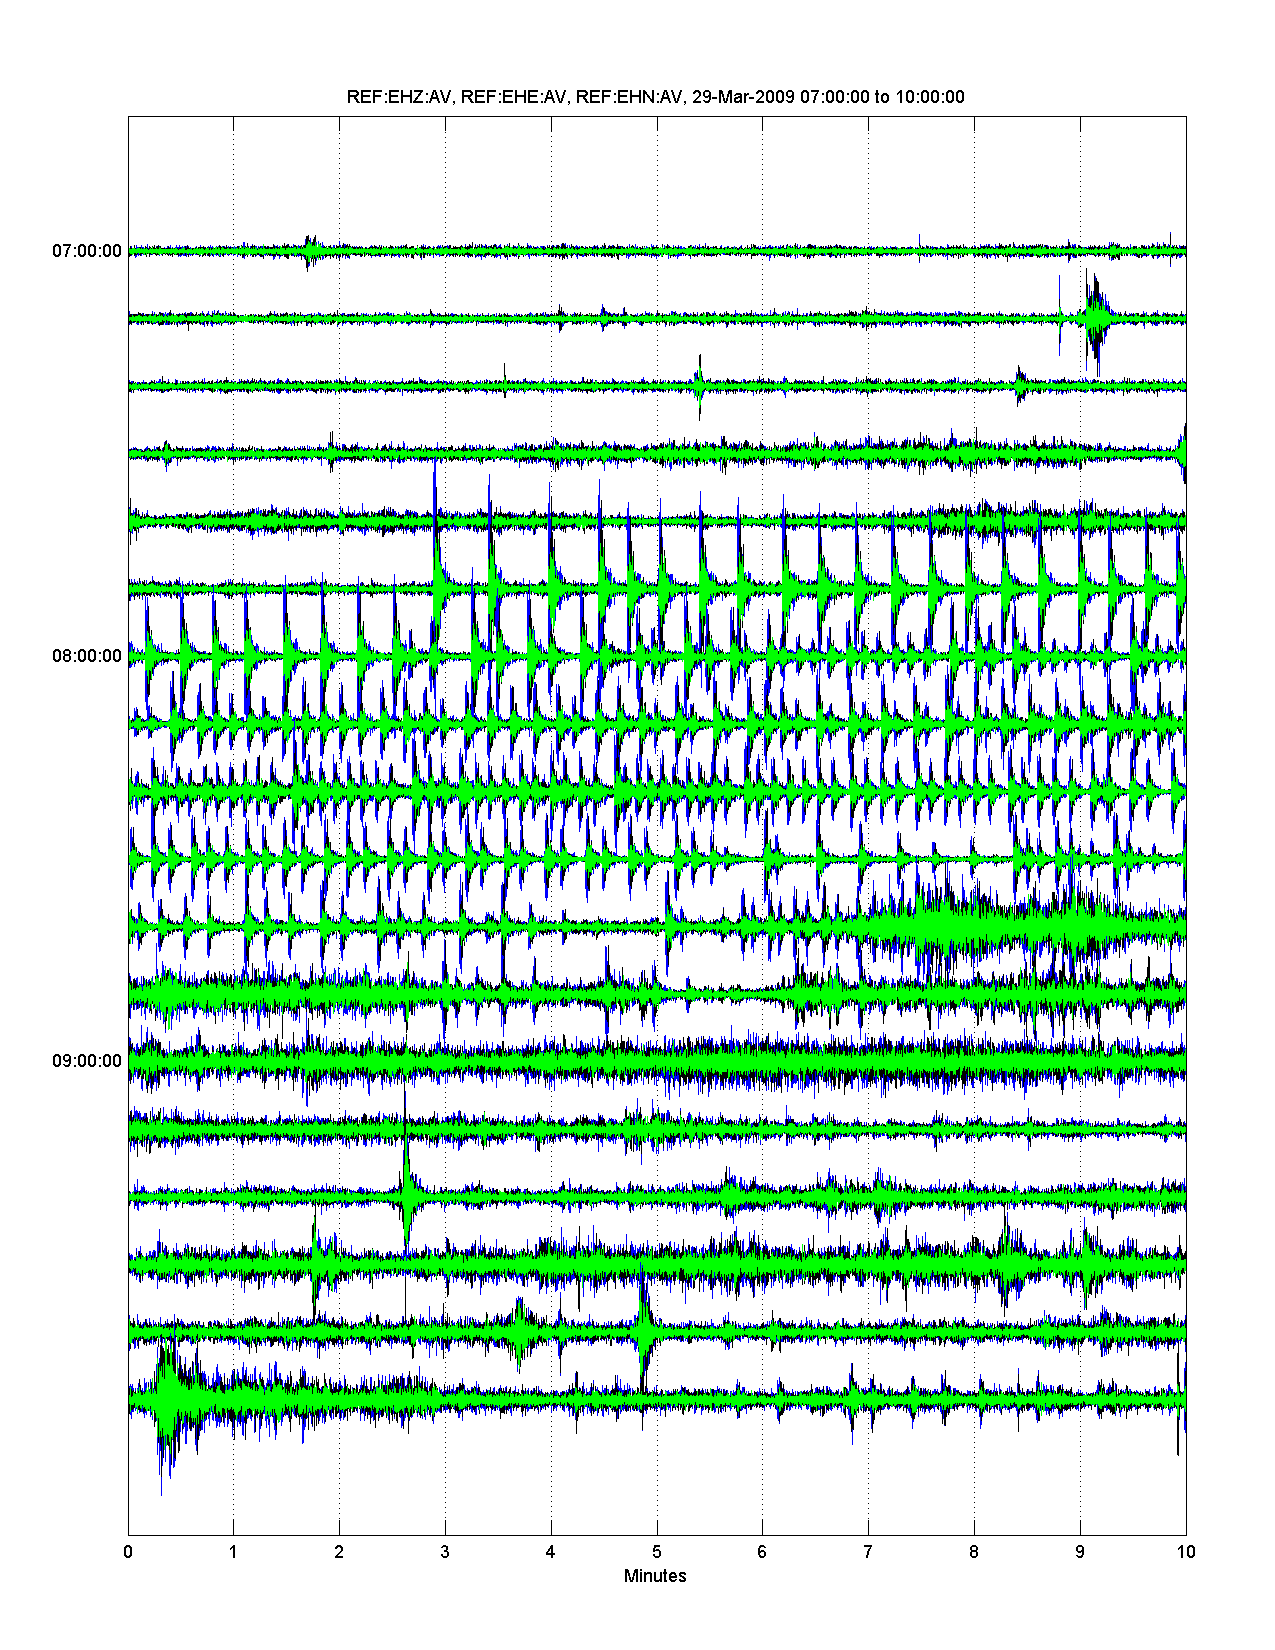
\includegraphics{hel_stack_1.png}}} 
\caption{Multi-waveform 'stack' display} 
\label{hel_stack_1}
\end{figure}

\clearpage

\subsection{Helicorder event overlay}

Helicorder can also be used to display discrete events from a waveform object. To do this, a set of event start/stop times (\mcode{sst1}) is required. Start/stop times can be manually picked, or can be the result of an auto-detection algorithm such as STA/LTA. 212 events are detected from the waveform data in Figure~\ref{hel_e_sst}. In our case, \mcode{sst1} is a 212x2 array of MatLAB times defining the begining and end of each event. Figure~\ref{hel_e_sst} displays the output from \mcode{build(helicorder(w,'mpl',15,'e_sst',sst1))} where \mcode{w} is broadband data from RDWB:BHZ from March 27, 2009 that has been band-pass filtered between 1 Hz and 10 Hz.

\begin{figure}[ht] 
\centerline{\scalebox{.6} {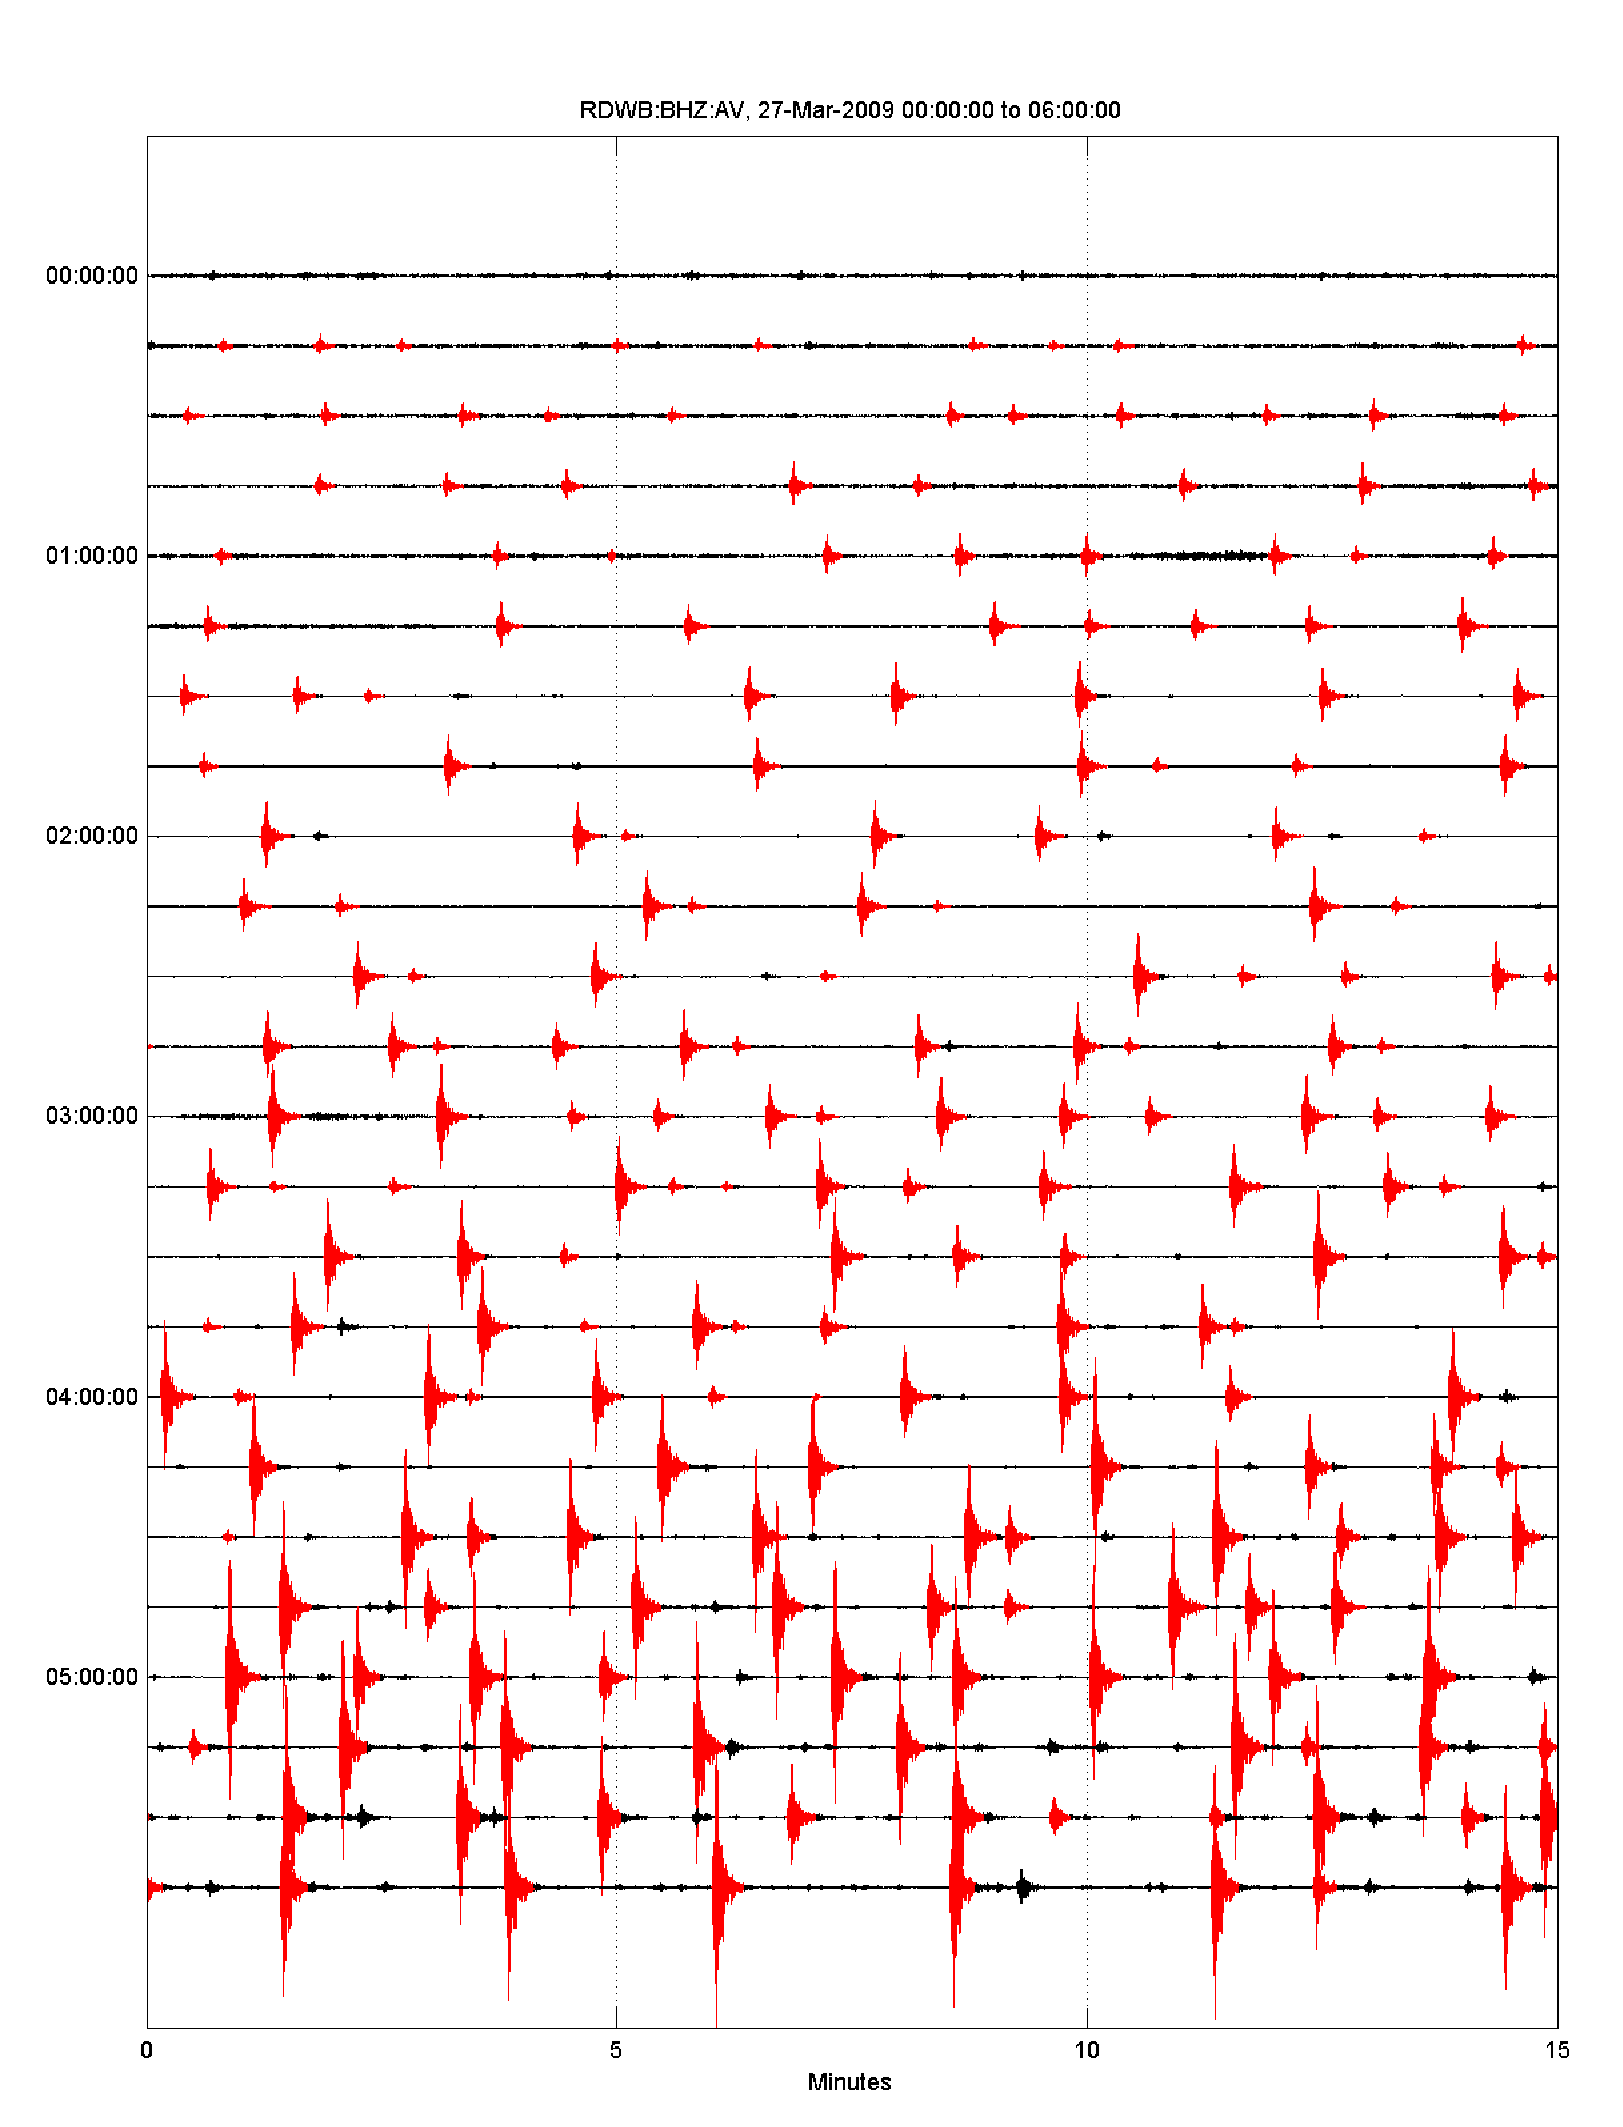
\includegraphics{hel_e_sst.png}}} 
\caption{Helicorder with event overlay} 
\label{hel_e_sst}
\end{figure}

\clearpage

\subsection{Helicorder VLP overlay example}

In the next example, \mcode{w} contains the unfiltered data from the previous event overlay example. Calling \mcode{build(helicorder(w,'mpl',15))} returns the following display:

\begin{figure}[ht] 
\centerline{\scalebox{.6} {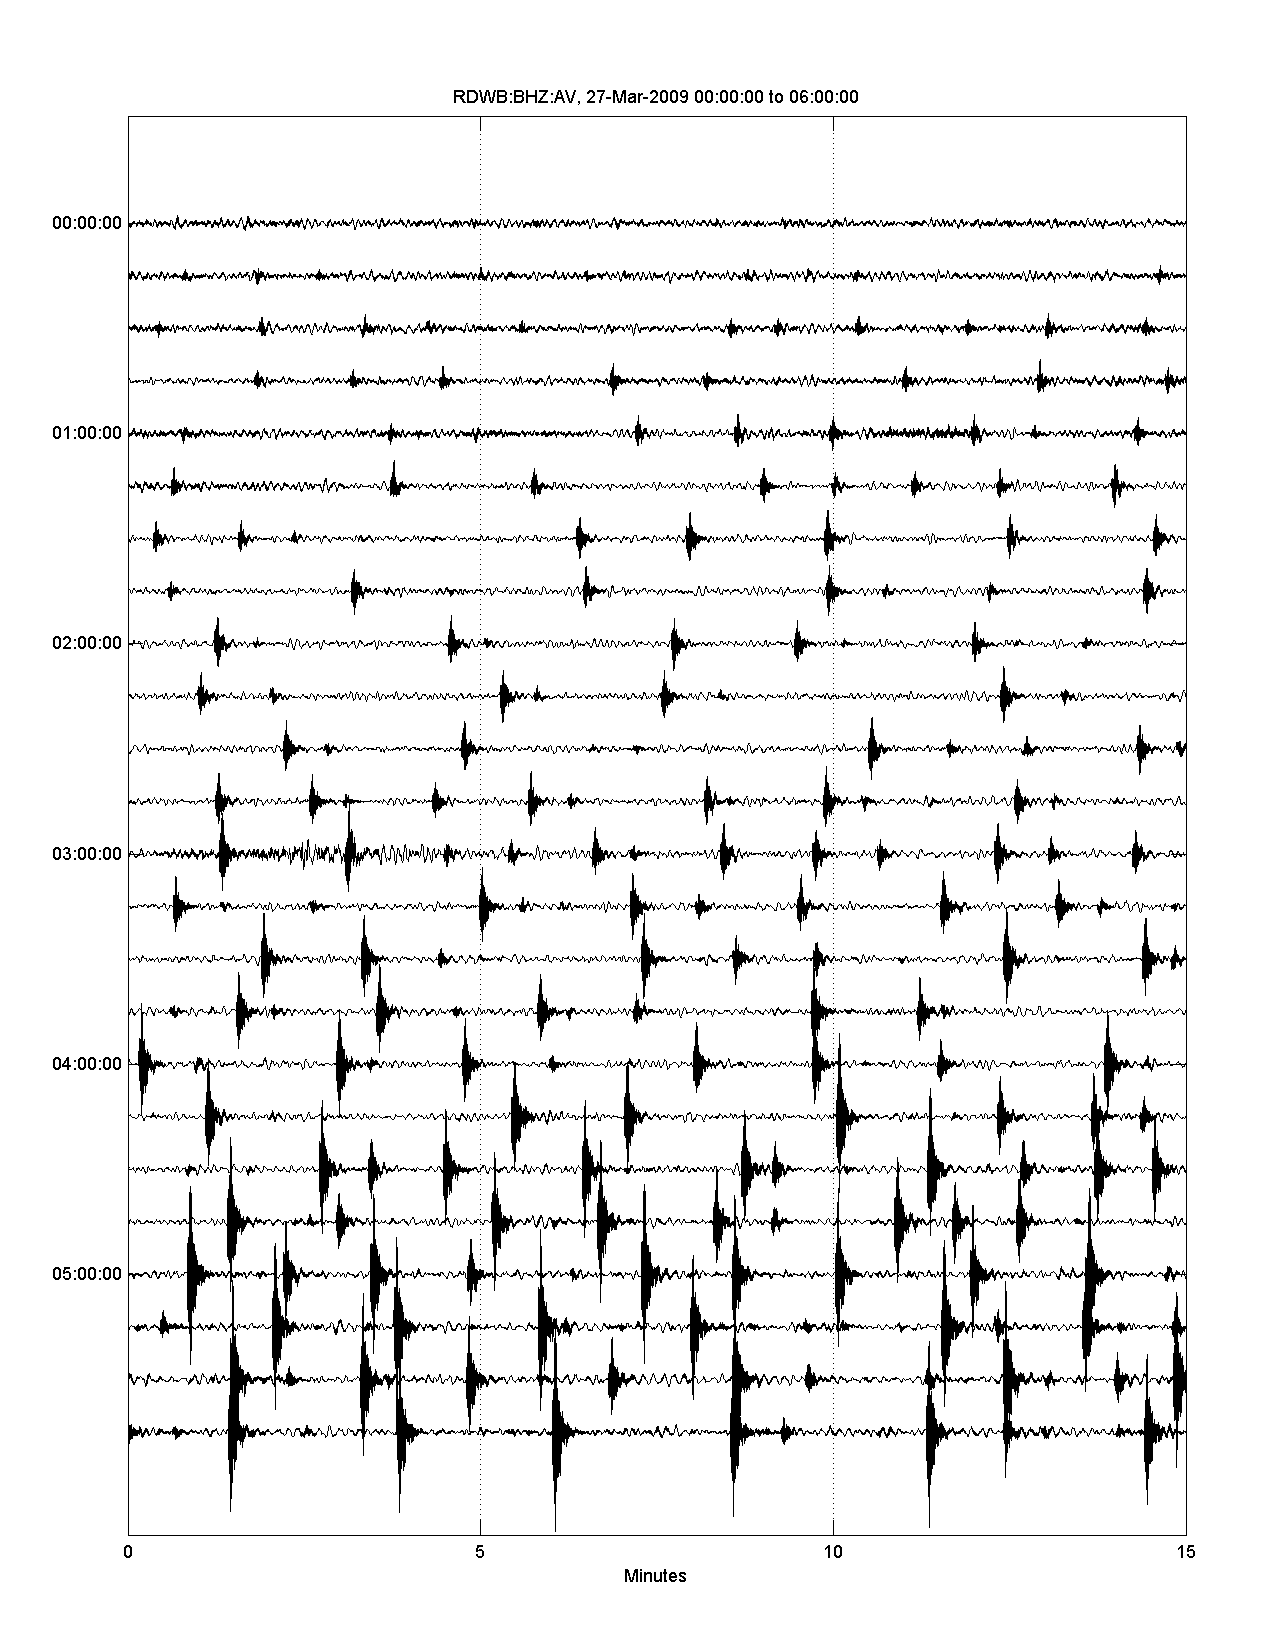
\includegraphics{hel_single_2.png}}} 
\caption{RDWB:BHZ helicorder} 
\label{hel_single_2}
\end{figure}
\clearpage

We suspect that there may be VLP energy in this data set, so we integrate \mcode{w} data to move from velocity to displacement. A second waveform \mcode{w_vlp} is created by filtering \mcode{w} over the VLP range (whatever you believe that might be). Next we combine \mcode{w} and \mcode{w_vlp} as follows: \mcode{w = [w w_vlp]}. This guarantees that VLP data is plotted on top of displacement data as seen in Figure~\ref{hel_stack_2}. We aren't satisfied with the default trace colors so we set them ourselves:  

\begin{lstlisting}
color = {[0 0 0],[1 0 0]}; % Normalized RGB value for black and red
build(helicorder(w,'mpl',15,'trace_color',color))
\end{lstlisting}


\begin{figure}[ht] 
\centerline{\scalebox{.6} {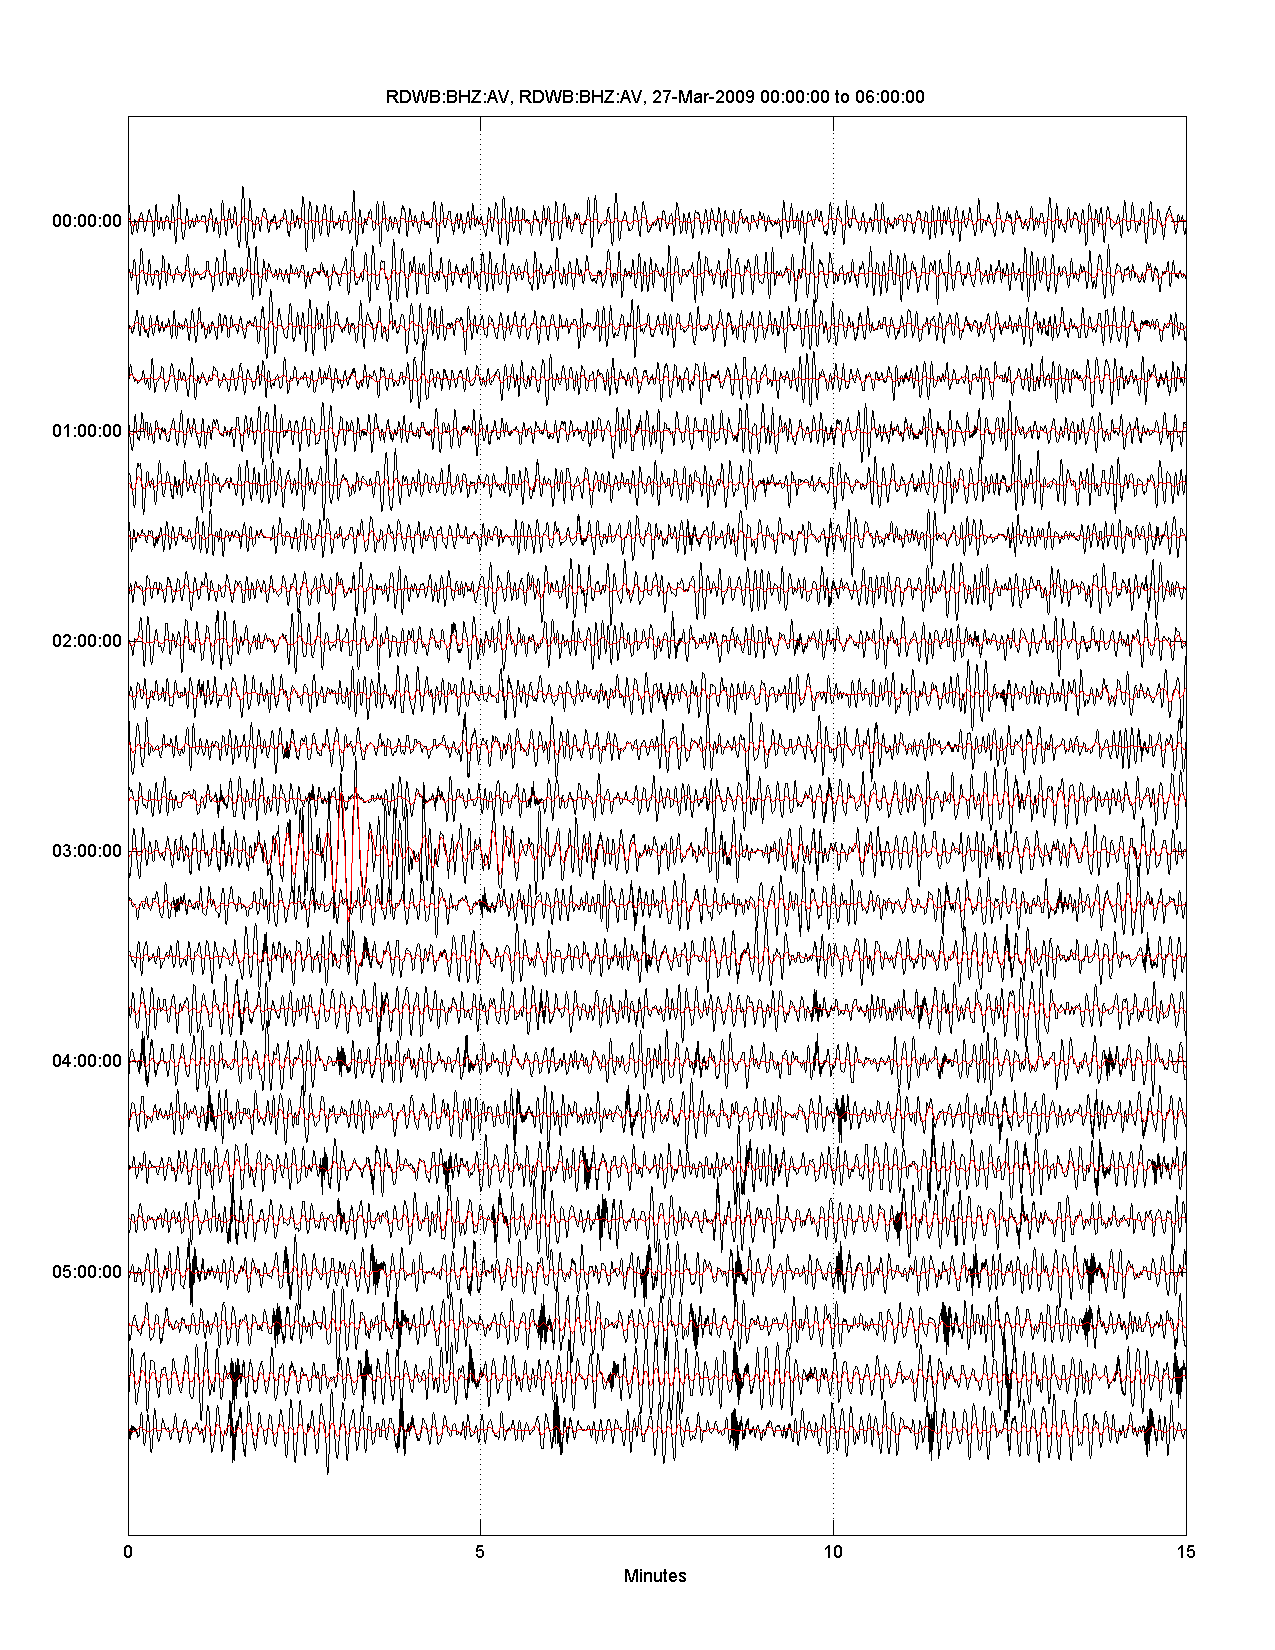
\includegraphics{hel_stack_2.png}}} 
\caption{Helicorder VLP overlay} 
\label{hel_stack_2}
\end{figure}

\clearpage

\subsection{Valid helicorder property name/value combinations}

\begin{itemize}
\item \mcode{e_sst} - Event Start/Stop Times \\
If wave contains only one wavefrom object, \mcode{e_sst} can be entered as an Nx2 array of matlab times. If there is more than one waveform in wave (M waveforms), \mcode{e_sst} must be a 1xM cell array, each cell containing Nx2 array of start/stop times. A single waveform can also have multiple sets of start/stop times as in a waveform with multiple event families. In this case \mcode{e_sst} should be entered as a 1xL cell array for a particular waveform (with L separate groups to be highlighted).
EXAMPLE: \mcode{h = helicorder(w,'e_sst',A)} where \mcode{w} is a 1x2 waveform object \\
\mcode{A} is a 1x2 cell array \\
\mcode{A(1,2)} is a 1x3 cell \\
\mcode{A(1,2)\{1\}} is a Nx2 numeric array \\
\mcode{A(1,2)\{2\}} is a Nx2 numeric array \\
\mcode{A(1,2)\{3\}} is a Nx2 numeric array \\
DEFAULT = [] (No events)

\item \mcode{mpl} - Minutes Per Line \\
single numeric value specifying number of minutes per helicorder line. (This applies to all waveforms in the helicorder)\\
DEFAULT = 10 

\item \mcode{trace_color} - Color Scheme of Trace Data\\
If \mcode{w} contains only one wavefrom object, \mcode{trace_color} can be entered as a 1x3 array of RGB values (between 0 and 1). For wave arguments longer than 1, \mcode{trace_color} should be entered as a 1xN cell array, each containing a 1x3 array of RGB values.

\item \mcode{event_color} - Color Scheme of Highlighted Event Data\\
Only use this property when \mcode{e_sst} property exists. \mcode{event_color} follows the same structure as \mcode{e_sst}. If wave contains only one waveform object, \mcode{event_color} can be entered as a 1x3 array of RGB values (between 0 and 1). For wave arguments longer than 1, \mcode{event_color} should be entered as a 1xN cell array, each containing a 1x3 array of RGB values. If multiple event sets exist for a single waveform, \mcode{event_color} must be specified accordingly.\\
EXAMPLE: \mcode{h = helicorder(w,'e_sst',A,'event_color',B)}\\
\mcode{A} is the same as the previous example\\
\mcode{B(1,1)} is a 1x3 RGB array\\
\mcode{A(1,2)} is a 1x3 cell\\
\mcode{A(1,2)\{1\}} is a 1x3 RGB array\\
\mcode{A(1,2)\{2\}} is a 1x3 RGB array\\
\mcode{A(1,2)\{3\}} is a 1x3 RGB array\\
DEFAULT = [] (No events)

\item \mcode{display} - Multi-Waveform Display Type\\
\mcode{'single'} - Used when there is only one waveform in wave. None of the multi-waveform display types can be set unless multiple waveforms are passed.\\
\mcode{'stack'} - Plots multiple waveforms over top of each other. (Multiple motivations could exist for wanting to display data in this way such as overlaying VLP energy).\\
\mcode{'alternate'} - Alternate through waveforms (grouped by time).\\
\mcode{'group'} - Plot all trace data in a waveform before starting the next (grouped by waveform source).\\
DEFAULT = 'single', 'alternate' (1 or multiple waveforms)

\end{itemize}

\clearpage

\subsection{Interacting with a helicorder figure}

The \mcode{build} fuction also provides a degree of interactivity with the helicorder figure. Clicking the cursor on any trace in the helicorder figure will call the function \mcode{traClick} from within \mcode{build}. The user can define what takes place after a helicorder trace line, or a highlighted event is clicked. By default, the GUI \mcode{sst_pick} is opened for the clicked waveform generating a minute-long waveform and spectral display.

\clearpage

\section{Event Detection Using STA/LTA}

The most common technique used in detecting discrete seismic events on both single and multiple stations is Short-Term Average, Long-Term Average Ratio (STA/LTA). In this approach, a short window of length $L_{sta}$ overlaps a longer window of length $L_{lta}$. The two windows share the same leading edge and are continuously updated as they are slid temporally through a seismic signal. An event is triggered when the time-averaged amplitude of the short data window $A_{sta}$ divided by the time-averaged amplitude of the long data window $A_{lta}$ exceeds a user-defined threshold $t_{on}$. When the ratio $A_{sta}/A_{lta}$ drops below a second user-defined threshold $t_{off}$, the detected event is considered to be over. Post-trigger discriminators are often used alongside this mechanism to either keep or discard the triggered events. Common examples of such discriminators are minimum allowable duration $DUR_{min}$ and minimum allowable root mean square $RMS_{min}$, criteria by which events that are too short or too low in amplitude respectively would be filtered out of the resulting set of events.

The use of STA/LTA is a simple and imperfect technique for automatically recording and quantifying discrete earthquakes. The algorithm doesn't begin to approach the abilities of the human brain in recognizing patterns, especially across a variety of different types of seismicity. To select tens of thousands of discrete events by hand, however, is less than practical. Speed is the primary advantage to using an automated approach. User-defined settings represent the controlled input of a system that can be tuned to optimize performance. On one side of the performance spectrum, STA/LTA sensitivity is set high, resulting in a very large array of detected events including an abundance of false triggers from seismic and telemetry noise. On the other end, we see a neat and small set of large amplitude events with many of the medium-sized and less impulsive earthquakes completely vacated. 

The function \mcode{sta_lta} implements this algorithm for waveform object inputs. Like many other functions in SEMS, \mcode{sta_lta} has a mandatory waveform input as well as a number of property values that can be customized by the user. The first is the STA/LTA Event Detection Parameters (EDP) which are contained in a 1x8 numeric array. Calibrabting EDP for a given station may require some trial and error. The order of these parameters along with descriptions are included in the code below, and a more in depth discussion on STA/LTA parameter setting can be found in \cite{trnkoczy-2002}.
\begin{lstlisting} 
l_sta = 1;     % STA window length (s)
l_lta = 8;     % LTA window length (s)
t_on = 2;      % STA/LTA trigger on threshold
t_off = 1.6;   % STA/LTA trigger off threshold
skip_int = 0;  % Skip ahead after end of event (s)
min_dur = 1.7; % Minimum event duration (s)
pre_t = 0;     % Added pre-event time (s) 
post_t = 0;    % Added post-event time (s)

your_edp = [l_sta l_lta th_on th_off skip_int min_dur pre_t post_t];
event_sst = sta_lta(w,'edp',your_edp) 
% The above EDP values are the default values,
% which makes the above code equivalent to:
event_sst = sta_lta(w); 
\end{lstlisting}

The user may also define the output type of \mcode{sta_lta} to be a waveform array as opposed to the default type (start/stop times). Someone interested in only examining events on a helicorder, or archiving times might choose the default. Returning events as a waveform array, however, can fascilitate post-detection descrimination or analysis. Examples of this might be event RMS, peak frequency, or cross-correlation. User-defined return type is demonstrated below.

\begin{lstlisting}
events = sta_lta(w); % returns events as start/stop times
events = sta_lta(w,'return','wfa'); % returns events as waveform array
\end{lstlisting}

\clearpage

If there exist periods in waveform \mcode{w} that the user wishes the STA/LTA algorithm to skip, then the 'skip' property can be used: \mcode{events = sta_lta(w,'skip',skip_sst)}. Here, \mcode{skip_sst} is a Nx2 array of start/stop times defining unwanted pieces of waveform \mcode{w}. These pieces may be calibration pulses, noise, or other artifacts. \mcode{sta_lta} will covert those periods to NaN values before event detection begins. When \mcode{sta_lta} encounters a section of NaN values, it simply advances the detection window forward in time until it is out of the NaN gap, then resumes detection.

The final property that can be specified by the user is post-trigger LTA window behavior. The first behavior, 'frozen', involves holding the position of the LTA window static while the STA window moves forward through time. In this case, the ratio $A_{sta}/A_{lta}(t)$ simply becomes a function of $A_{sta}(t)$. In the second behavior, 'continuous', the LTA window advances with the STA window and both are updated in the same fashion as before an event trigger occurred. Both of these LTA settings offer some distinct advantage over the other, but either can also incur undesired effects. The frozen setting has the advantage of capturing more completely the coda from events, especially those higher in energy with longer durations. Continuous LTA behavior will often flip an event trigger off prematurely once a significant amount of the LTA window overlaps the event. This can especially be an issue when $L_{lta}$ is not long. The primary disadvantage of the frozen setting, however, is the possibility for turning a trigger on that can't be turned off. The presence of spiky and noisy data, data gaps, and a background seismic level that changes rapidly over a short duration can initiate a trigger in the presence of a low $A_{sta}$ making it difficult for the $A_{sta}/A_{lta}$ value to drop below $t_{off}$.

The third and final post-trigger LTA window behavior is called 'grow' and represents a compromise between both 'frozen' and 'continuous'. In this scheme, the tail end of the LTA window is frozen, and the leading-edge of the LTA window is continuous. This means that $L_{lta}$ is expanding and $A_{lta}$ is averaging more and more data. When the trigger is turned off, the LTA resumes its original length. The default method is 'frozen'. All three methods are invoked in the code below, then displayed 

\begin{lstlisting}
e_1 = sta_lta(w,'lta_mode','frozen');     % Default, equivalent to: e_1 = sta_lta(w)
e_2 = sta_lta(w,'lta_mode','continuous'); % Continuous mode
e_3 = sta_lta(w,'lta_mode','grow');       % Grow mode
w = [w w w];                        % Replicate w for helicorder plotting
e = {e_1 e_2 e_3};                  % Place events in cell array, length(w)=length(e)
build(helicorder(w,'e_sst',e))      % helicorder magic
\end{lstlisting}

\begin{figure}[ht] 
\centerline{\scalebox{.8} {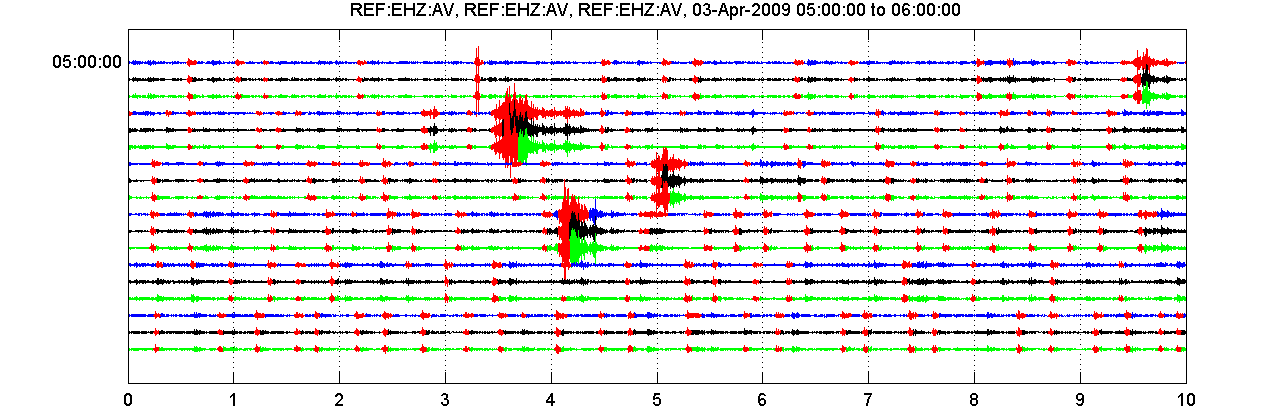
\includegraphics{hel_lta_modes.png}}} 
\caption{'Frozen', 'Continuous',and 'Grow' LTA modes} 
\label{hel_lta_modes}
\end{figure}

\clearpage

\section{Event Pick}

The GUI \mcode{event_pick} can be used to manually pick event start/stop times from a waveform object \mcode{w}. The GUI creates a split display of waveform trace data and waveform spectral data seen in Figure~\ref{event_pick}. The user can rapidly scroll through \mcode{w} using the left and right arrow keys, as well as zoom in and out with the up and down arrow keys. Each pair of mouse clicks will highlight an event to be later output by the GUI. The command \mcode{sst1 = event_pick(w)} will open the GUI seen in Figure~\ref{event_pick}.
\begin{figure}[ht] 
\centerline{\scalebox{.5} {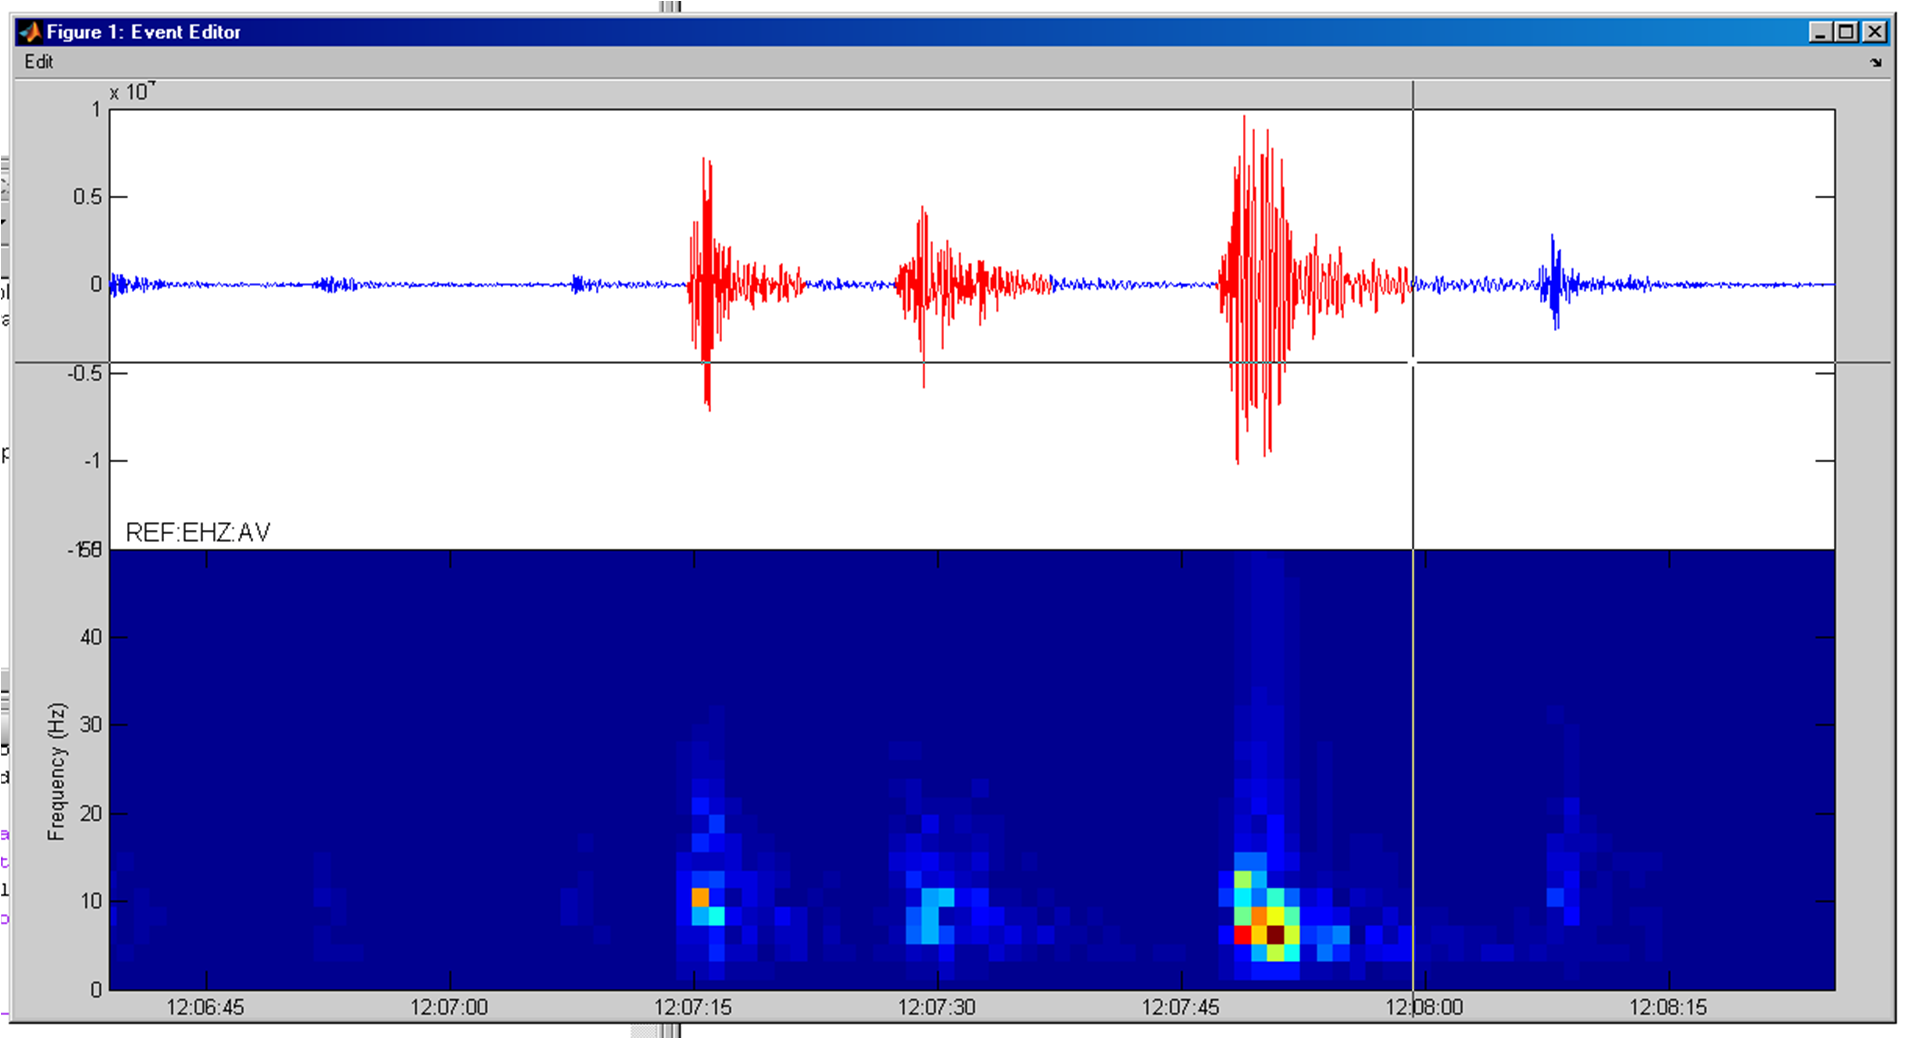
\includegraphics{event_pick.png}}} 
\caption{Event Pick GUI} 
\label{event_pick}
\end{figure}
\clearpage

\section{Event Metrics}
A few metrics are available in SEMS by which a single numeric value can be used to describe a particular event. Root Mean Square (RMS) is one such metric that you are probably familar with. This is an average measure of the energy within the event waveform. SEMS offers a way to quickly compute, display, and interact with this information. All of the event metric functions can provide the user with a numerical array output, or can directly generate an interactive figure. As with the helicorder figure, data points in any event metric function can be clicked to execute code from within that function. For a large set of automatically detected events, an event metric plot might provide relevent seismic trend information. It also provides a quick view of outlier data. The following four metrics are currently available in SEMS:
\begin{itemize}
\item \mcode{event_rms} - Event RMS ()\\
\mcode{erms = event_rms(e_wfa,op)} 
\item \mcode{event_space} - Inter-event spacing (Temporal distace between event start times)\\
\mcode{es = event_space(e_sst,unit,op)} 
\item \mcode{peak_freq} - Peak Frequency (Most energetic single frequency present via the Discrete Fourier Transform)\\ 
\mcode{pf = peak_freq(e_wfa,op)} 
\item \mcode{freq_index} - Frequency Index (Ratio of low to high frequency content as defined in \cite{buurman-west-2010})
\end{itemize}

\clearpage

\bibliography{SEMS}{}

\bibliographystyle{ieeetr}

\end{document}

